% !TeX program = pdflatex
% !TeX encoding = UTF-8

%==============================
% Splatone Preprint (Skeleton)
%==============================

\documentclass[11pt,a4paper]{jlreq}

%--------- Packages ----------
\usepackage[T1]{fontenc}
\usepackage[utf8]{inputenc}
\usepackage{lmodern}
\usepackage{amsmath,amssymb,amsthm}
\usepackage[dvipdfmx]{graphicx}
\usepackage{tikz}
\usetikzlibrary{arrows.meta, positioning}
\usepackage{authblk}
\usepackage{url}
\usepackage{hyperref}
\usepackage{geometry}
\geometry{margin=25mm}
\usepackage{listings}
\usepackage{xcolor} % 色を使う場合
\usepackage{svg}

\svgpath{{figures/}}
%\svgsetup{inkscapelatex=true, inkscapepath={C:/Program Files/Inkscape/bin/}}

\lstdefinestyle{commandline}{
  basicstyle=\ttfamily\small,
  backgroundcolor=\color{black!5},
  frame=single,
  columns=fullflexible,
  keepspaces=true,
  escapeinside={} % ★ ここがポイント:エスケープ無効
}

\lstnewenvironment{commandline}[1][]{
  \lstset{style=commandline,#1}
}{}

%--------- Meta data ----------
\title{Splatone crawler: ジオソーシャルデータの収集・可視化のための汎用ツール}

% TODO: 著者情報を埋めてください
\author[1]{横山昌平}
\affil[1]{東京都立大学, 東京都日野市旭が丘6-6}

\date{\today}

%--------- Document ----------
\begin{document}

\maketitle

\begin{abstract}
  % このツール Splatone の概要を1段落で記述して。
  位置情報付き画像コレクションは,観光行動や都市空間の理解に有用な情報源として注目されているが,その空間的・時間的な不均一性や膨大な量により,単純な地図表示では全体の傾向把握が困難である.
  本研究では,位置情報付き画像の色彩情報と位置情報を統合的に扱う可視化ツール Splatone Crawler を提案する.
  Splatone Crawler は,知覚的距離に基づいた自動カラーパレット生成と,地理空間上の Voronoi 分割,クラスタリング,グリッド集計など複数の可視化手法を組み合わせることで,ジオタグ位置分布だけでなく,カテゴリごとの空間配置を直感的に把握できることを目指す.
  また,ツール本体はプロバイダーと visualizer を差し替え可能な拡張機構を備えており,新たなデータソースや可視化手法を容易に追加できる点も特徴である.
  提案手法の実装系は GitHub および NPM にて公開されており,誰でも利用可能である.
  本論文ではそのシステム構成、利用方法、および利用事例を示す.
\end{abstract}

\section{はじめに}
近年,位置情報付きソーシャルデータを分析・活用するための基盤は整いつつあるものの,(1) カテゴリ(キーワード集合)間の空間的差異を同一フレームで比較しづらい,(2) 可視化手法ごとの前処理(グリッド化,クラスタリング等)が個別実装になり再利用性が低い,(3) 高視認性彩色と地理的構造(密度・境界・混在度)を統合した視覚表現が不足している,といった課題が残されている.特に複数キーワードを束ねたカテゴリ単位での比較は,単純な点描画だけでは分布の偏り・重なり・局所的特徴を解釈しにくく,分析者がズーム・パンを繰り返す探索的操作に依存しがちである.


本研究で提案する Splatone Crawler は,これらの課題に対処するため,クローリングから色特徴抽出・空間集約・複数可視化への受け渡しを一貫パイプライン化し,かつプロバイダー/visualizer 拡張を前提とした枠組みを提供する.本ツールの主な特徴と貢献を以下に整理する.
\begin{itemize}
  \item ワーカープロセスを介した非同期クローリングによる大規模データ収集の効率化
  \item GeoJSON形式によるデータモデルの統一化と可視化手法間の連携容易化
  \item カテゴリ(複数キーワード集合)概念の導入による柔軟な OR 検索とカテゴリ別比較
  \item 知覚距離に基づく自動パレット生成の統合(色の一貫した割当)
  \item 六角グリッド・Voronoi・密度(KDE)・クラスタ(DBSCAN)・割合円グラフ等,異なる空間表現の並列提供
  \item 可視化/取得対象(Provider, Visualizer)のモジュール化による第三者拡張性
  \item コマンドライン起動とブラウザ UI の即時連携による試行錯誤的探索支援
\end{itemize}

これにより,単一手法では捉えにくかった「カテゴリ間の空間的入れ替わり」「局所的優勢の分布可視化」「高密度点群区域の内部構造」などを多面的に観察できる.以降では関連研究を概観した後(第\ref{sec:related}章),データモデルと全体構成(第\ref{sec:overview}章),色彩情報を活用する可視化手法群(第\ref{sec:colorviz}章),拡張を可能にする実装上の工夫(第\ref{sec:implementation}章),具体的利用事例(第\ref{sec:usecases}章),最後に考察と今後の課題(第\ref{sec:discussion},\ref{sec:conclusion}章)を述べる.

近年,Flickr をはじめとする写真共有サービスや,SNS 上で投稿される写真には位置情報が付与されることが一般的になり,大規模な位置情報付き画像コレクションが容易に取得できるようになっている.
これらのデータは,人々の移動や観光行動,都市空間の使われ方など,従来の調査では把握が難しかった現象を分析するための有力な情報源として注目されている.
一方で,位置情報付き画像は空間的・時間的に不均一かつ量が膨大であり,単純に地図上にマーカとして表示するだけでは,全体の傾向や特徴的なパターンを把握することが難しい.

こうした課題に対し,地理空間上での分布や時空間パターンを可視化・解析するための手法がこれまでに多数提案されている.
例えば,K{\'a}d{\'a}r ら\cite{kadar2013wheredotouristsgo} は観光客によって撮影された位置情報付き写真の空間分布を解析し,観光地内での人気エリアや動線を明らかにしている.
また,Kisilevich ら\cite{kisilevich2010eventbased} は Flickr および Panoramio の画像を用いてイベントに関連する人々の活動パターンを抽出し,クラスタリング結果を地図上に可視化している.
これらの研究は,位置情報付き写真が観光や都市解析に有用であることを示しているが,可視化の多くは密度マップやクラスタ境界の表示に留まっており,色やカテゴリ情報を手がかりにした多面的な可視化環境は必ずしも十分ではない.

本研究では,位置情報付き画像コレクションの色彩情報と位置情報を統合的に扱う可視化ツール Splatone Crawler を提案する.
Splatone Crawlerは,知覚的距離に基づいた自動カラーパレット生成と,地理空間上の Voronoi 分割,クラスタリング,グリッド集計など複数の可視化手法を組み合わせることで,ジオタグ位置分布だけでなく,カテゴリごとの空間配置を直感的に把握できることを目指す.
また,ツール本体はプロバイダー/visualizer を差し替え可能な拡張機構を備えており,新たなデータソースや可視化手法を容易に追加できる点も特徴である.

なお、SplatoneはGitHub \footnote{https://github.com/YokoyamaLab/Splatone}およびNPM \footnote{https://www.npmjs.com/package/splatone}にて公開されており、誰でも使う事が可能となっている。

本論文の構成は次のとおりである.
第\ref{sec:related}章では,位置情報付き写真の可視化および分析に関する関連研究を概観する.
第\ref{sec:overview}章では,Splatone のデータモデルとシステム構成を説明する.
第\ref{sec:colorviz}章では,本研究で実装したカラーベースの可視化手法と,各 visualizer の役割について述べる.
第\ref{sec:implementation}章では,実装上の工夫や拡張機構について説明し,第\ref{sec:usecases}章で利用事例を示す.
最後に,第\ref{sec:discussion}章および第\ref{sec:conclusion}章で考察と結論を述べる.

\section{関連研究}
\label{sec:related}
位置情報付き写真を利用した可視化および分析に関する研究は,観光行動の解析,都市空間の理解,イベント検出など多様な文脈で行われている.
K{\'a}d{\'a}r ら\cite{kadar2013wheredotouristsgo} は,Flickr などから収集した位置情報付き写真を用いて,観光客がどこへ行くのかを可視化し,観光地における人気スポットや移動パターンを明らかにした.
彼らは写真の空間分布を地図上に表示しつつ,滞在時間や移動経路を解析することで,観光行動の偏りやホットスポットを定量的に評価している.

Kisilevich ら\cite{kisilevich2010eventbased} は,Flickr および Panoramio の位置情報付き画像コレクションに対しクラスタリングを適用し,イベントに関連する人々の活動パターンを抽出する手法を提案した.
クラスタ境界を凸包として可視化することで,特定イベントに紐づく空間的な広がりや集積度を地図上で把握できる.
Hu ら\cite{hu2015extractingAOI} は,複数都市の位置情報付き写真から,都市内の関心領域(Area of Interest)を抽出し,土地利用との関係を分析している.
Lee ら\cite{lee2014exploration} は,データマイニング手法を用いて位置情報付き写真のクラスタリングやパターン抽出を行い,地理空間的な利用パターンの理解に貢献している.

これらの研究はいずれも,位置情報付き写真が観光・都市解析の有効な情報源であることを示すとともに,空間分布やクラスタ構造の可視化に主眼を置いている.
一方で,写真に含まれる色やカテゴリといった視覚的特徴を,地理空間上の表現と密接に結びつけて対話的に探索できる汎用ツールはまだ限られている.
本研究の Splatone は,色彩情報と空間情報を同時に扱う複数の visualizer を統合的に提供する点で,既存研究を補完する可視化環境を目指している.

本研究で採用するボロノイ分割は,空間点集合から局所的勢力圏(最近領域)を定義し密度勾配や遷移境界を可視化する代表的手法であり,基礎理論と応用を体系化した Okabe らの著作\cite{okabe2000spatial}が広く参照されている.

格子集約系では等間隔正方格子より方向バイアスが少なく近傍関係が均質な六角ビニング\cite{carr1987hexbin}が大量点群の密度とカテゴリ比率表示に有効とされる.連続的密度場の推定にはカーネル密度推定(KDE)が用いられ,帯域幅選択やスムージングの統計的基盤は Silverman\cite{silverman1986density} により整理された.
クラスタ的構造の抽出と境界可視化にはノイズ耐性を持つ密度ベース手法 DBSCAN\cite{ester1996dbscan} が頻用され,観光・都市写真分布の局所集積検出に適用されている.

さらに点群のスケール非依存な空間パターン評価には Ripley の K 関数\cite{ripley1976second} が用いられ,K 曲線とランダム基準の差異を併置することで過密・過疎領域の多尺度的特徴を補助的に説明する可視化が提案されている.これら手法を組み合わせることで,単一表示では捉えにくい境界・密度・カテゴリ混在度を多面的に把握可能となる.

本論文では、それらこれまでの可視化手法を統合・複合的に利用できる他、プロバイダー/visualizer アーキテクチャにより第三者による機能拡張も容易である。著者自身も六角形格子と円グラフを組み合わせて複数のカテゴリに跨ったヒートマップを同一地図上に可視化するMajority Hexを提供している。
\section{システムの概要}
\label{sec:overview}

\subsection{用語定義}

\subsubsection{Splatone Crawler}

提案するシステムであり、SNSから複数のキーワードでジオタグ付きデータを検索し、キーワード毎の分布の違いを分析するために効果的な可視化を行う。

\subsubsection{キーワードとカテゴリ}

キーワードはソーシャルデータの検索に用いる単語の事である。例えばFlickrから森林の写真と海岸の写真の撮影位置を可視化したい場合、森林や海岸をキーワードどして指定すればよい。

ただし検索したい対象は一語のみで得られるとは限らない、例えば森林についてもう少し幅広く写真を集める場合、ジャングルやタイガ等のキーワードでも検索し、結果
一緒に扱いたい、すなわちOR検索をしたい場合が多い。本システムでは、カテゴリという概念をもちいてそれを実現している。カテゴリとは複数のキーワードを束ねる概念であり、ラベルを付ける事ができる。森林、ジャングル、タイガというキーワード群のラベルとして、例えば緑地というラベルを付ける事ができる。ラベルはあくまでキーワード群を識別するためのものであり、検索やクローリングには用いられない。

\subsubsection{Provider}

Splatone Crawlerはジオソーシャルデータに特化したクローラーであるが、集める対象は限定されず、Providerとして第三者が提供する事も可能である。現時点では画像共有サイトFlickrのみに対応している。

\subsubsection{Visualizer}

Visualizerは可視化手法をパッケージ化したものであり、これも第三者が任意の可視化手法を追加する事が可能である。拡張アーキテクチャにより、Visualizerはメインルーチンを侵食する事なく、サーバ側処理とブラウザ側処理を記述する事ができ、目的に応じて処理を配置する事ができる。

\subsection{Splatone Crawler CLI}
% この説ではCLIの仕様について述べる

Splatone CrawlerはJavaScrtiptにより実装されており、Command Line Interface (CLI)で起動するとWebサーバを立ち上げた後、Webブラウザを自ら立ち上げて、サーバ・クライアント型のシステムとして動作する。サーバ側ではSNSからのクローリングや可視化のための前処理を行い、地図上での可視化はWebブラウザ側で行う。また、npxによる起動に対応しているため、node.jsの環境さえ準備すれば、インストール等の環境構築は一切不要である。

さらに、ProviderとVisualizerという二系統のアドオン機能を持ち、複数のジオソーシャルデータ、複数の可視化手法に対応している。Providerはデータを集める対象となるサービス毎に構成し、現在のバージョンではFlickrのみに対応しているが、アーキテクチャはオープンである。

Visualizerはクローリングしたジオタグ付きデータを地図上に描画するための機能であり、これもサードパーティによる追加が可能である。現在は以下の可視化手法を実装している。

\begin{itemize}
    \item Bulky: クロールした全てのジオタグを小さな点で描画する
    \item Marker Cluster: 密集しているジオタグをクラスタリングしてまとめて表示する
    \item Pie Charts: Hex Gridに基づく可視化。セル中心にカテゴリ割合のPie Chartを描画し、カテゴリごとに半径を可変
    \item Majority Hex: HexGridの各セルをセル内で最頻出するカテゴリの色で彩色
    \item Heat: KDEによるヒートマップ
    \item Pie Charts: 円グラフグリッド
    \item Voronoi: HexGrid単位で集約したジオタグからVoronoiセルを生成し、各Hexのポリゴンでクリップして表示
    \item DBSCAN: ジオタグをDBSCANクラスタリングし、各クラスタの凸包をポリゴンとして表示
\end{itemize}

例として以下に最小構成のコマンドを記す。このコマンドでは写真共有サイトFlickrから撮影位置の緯度経度が付与された写真をクローリングし、地図上にマップする。なお、\texttt{--p-flickr-APIKEY}はFlickrのAPIキーであり、各自で取得したものに置き換える必要がある。

\begin{commandline}
npx -y -p splatone@latest crawler -p flickr -k "canal,river|street,alley|bridge"\
--vis-bulky --p-flickr-APIKEY="aaaaaaaaaaaaaaaaaaaaaaaaaaaaaaaaa"
\end{commandline}

コマンドを実行すると、Webブラウザが立ち上がり地図が表示される。ここで任意の場所を矩形ツールで指定しStart Crawlingボタンを押下する事で、クローリングが開始される。しばらくたつと当該領域の指定したキーワードを持つジオタグ付き写真の収集が完了し、地図上に表示される。

コマンドを実行すると、Webブラウザが立ち上がり地図が表示される。ここで任意の場所を矩形ツールで指定しStart Crawlingボタンを押下する事で、クローリングが開始される。しばらくたつと当該領域の指定したキーワードを持つジオタグ付き写真の収集が完了し、地図上に表示される。

コマンドを実行すると、Webブラウザが立ち上がり地図が表示される。ここで任意の場所を矩形ツールで指定しStart Crawlingボタンを押下する事で、クローリングが開始される。しばらくたつと当該領域の指定したキーワードを持つジオタグ付き写真の収集が完了し、地図上に表示される。

コマンドを実行すると、Webブラウザが立ち上がり地図が表示される。ここで任意の場所を矩形ツールで指定しStart Crawlingボタンを押下する事で、クローリングが開始される。しばらくたつと当該領域の指定したキーワードを持つジオタグ付き写真の収集が完了し、地図上に表示される。

\begin{figure}[h]
  \centering
  \includesvg[width=0.7\textwidth,inkscapelatex=false]{overall}
  \caption{Splatone Crawler の全体構成}
  \label{fig:architecture}
\end{figure}

\begin{figure}[h]
  \centering
  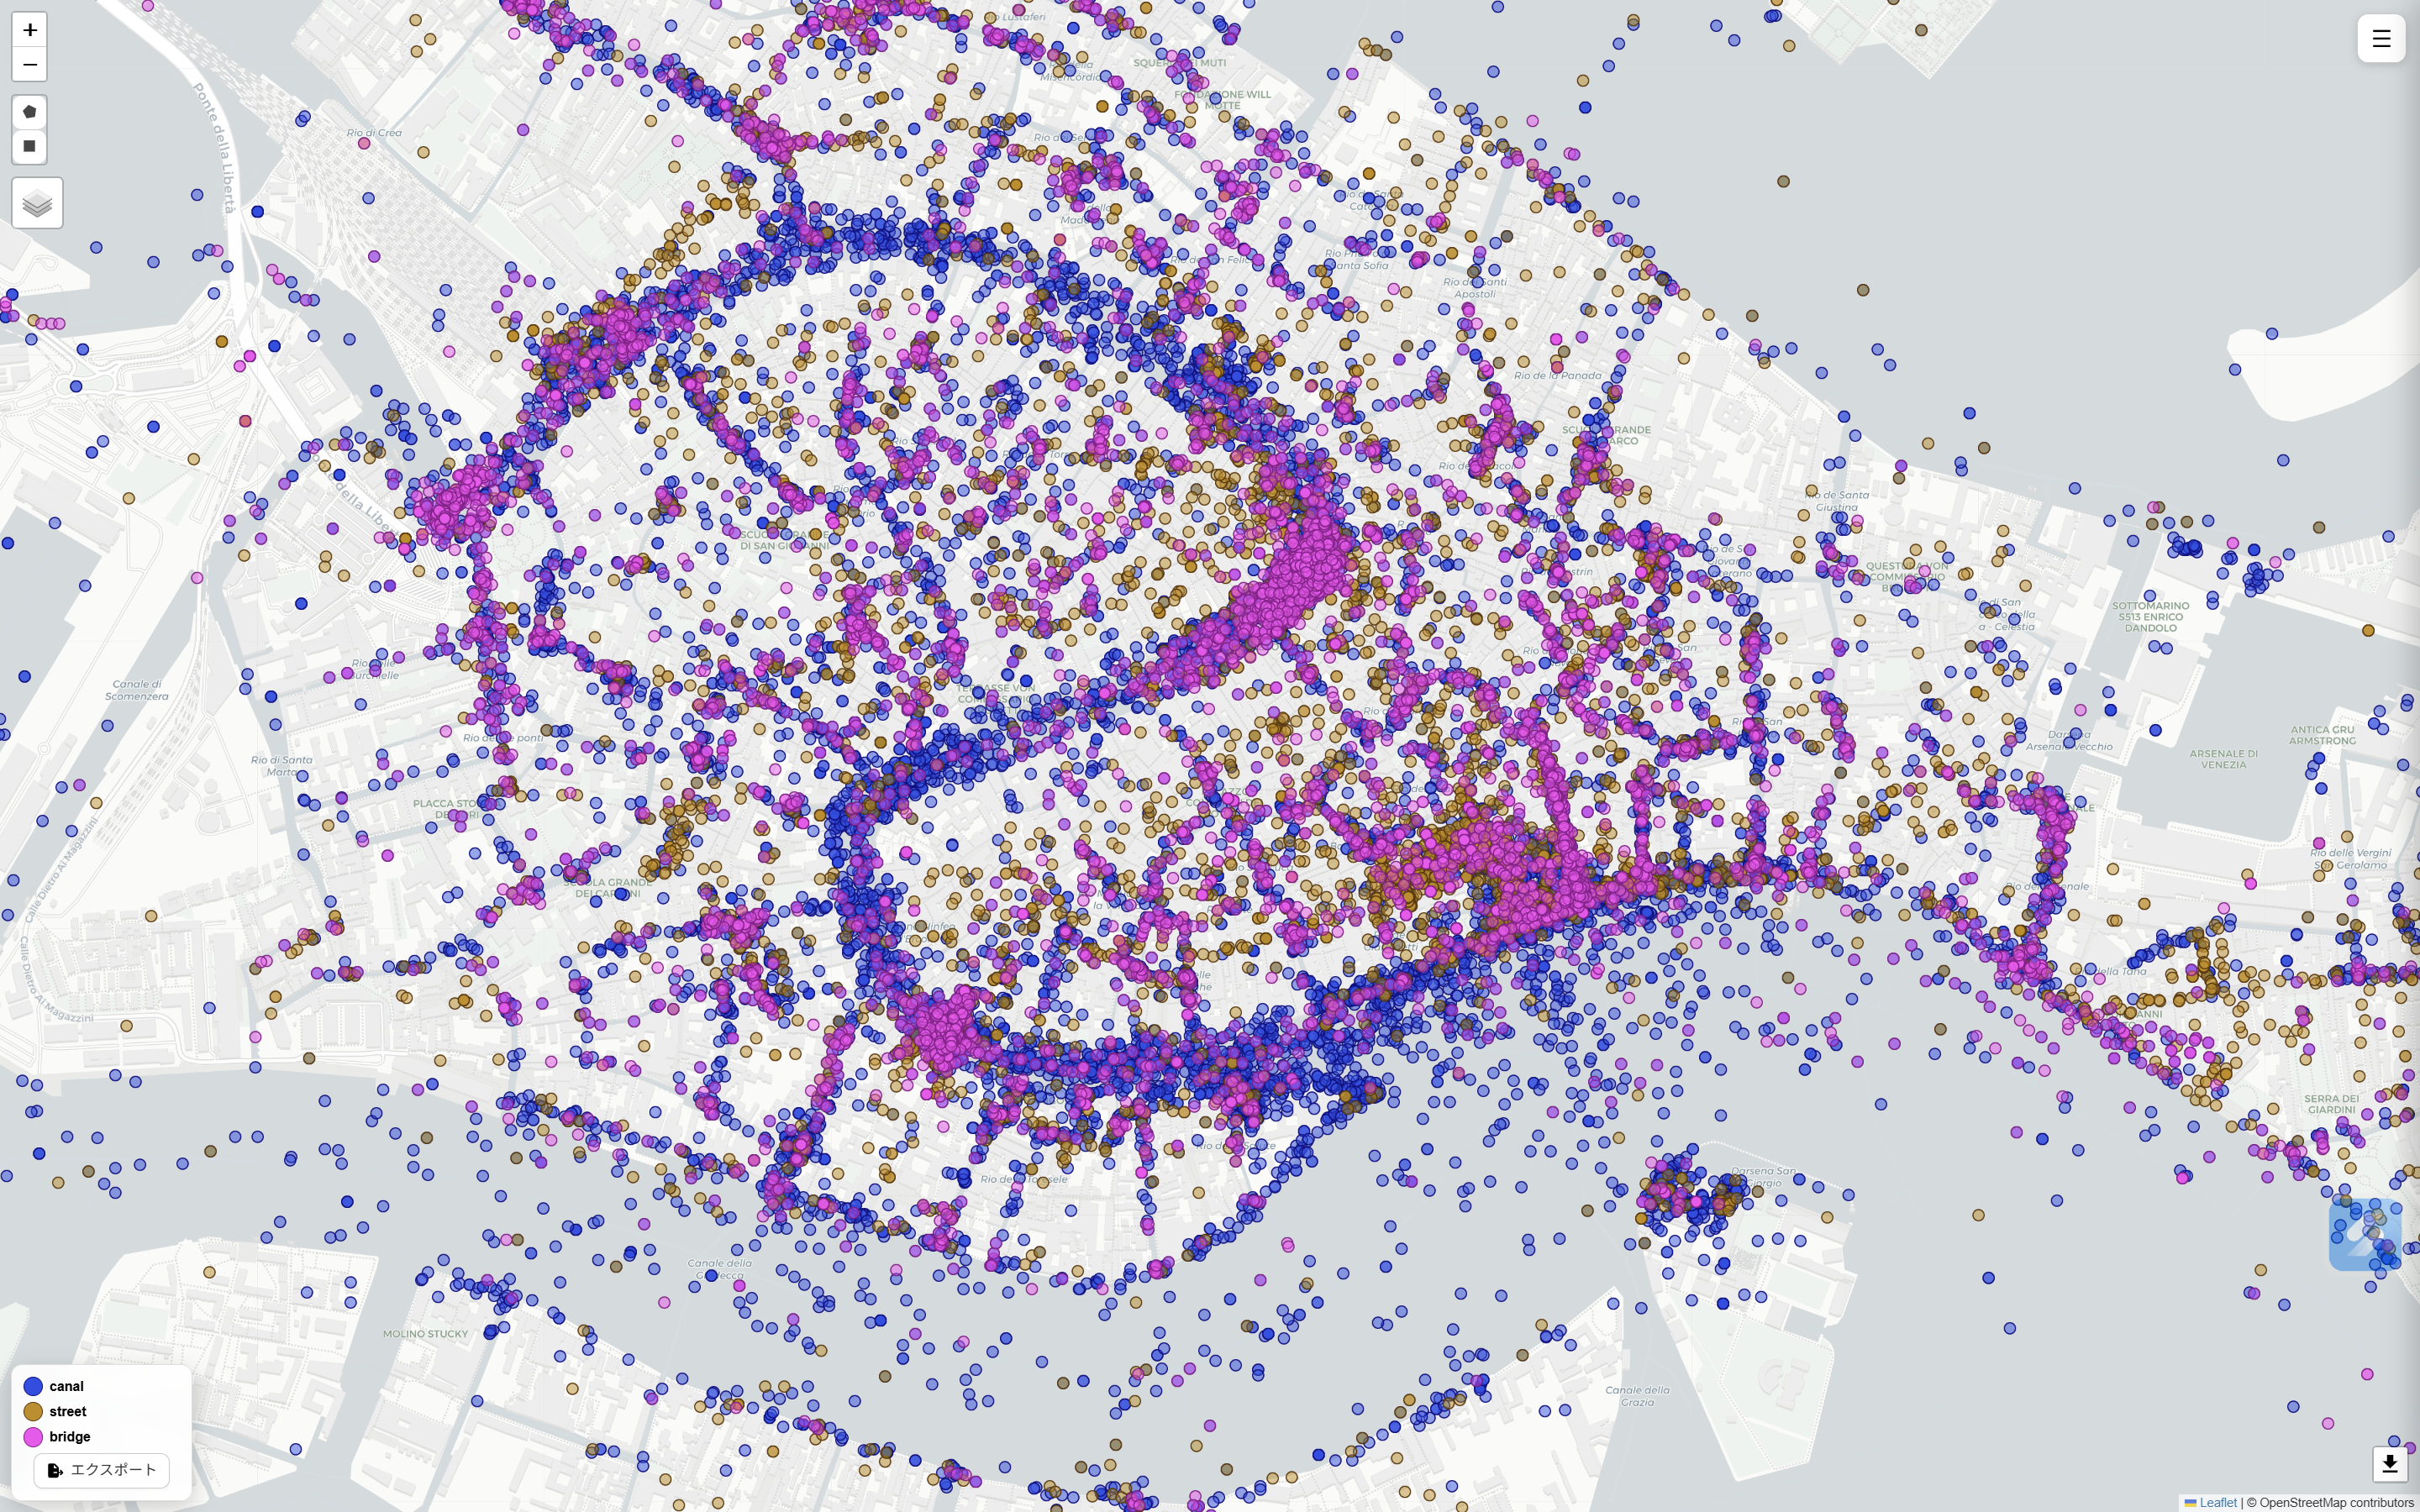
\includegraphics[width=0.5\textwidth]{figures/result_venezia_bulky.png}
  \caption{ベネチアの結果例(bulky版)}
  \label{fig:venezia_bulky}
\end{figure}

\subsection{Data Model}
% 画像, メタデータ (位置, タグなど) の扱い

\subsection{Architecture}
Splatone の全体構成を図~\ref{fig:architecture} に示す.
本ツールは大きく,(1) 画像およびメタデータを取得する Crawler 層,(2) 取得データに対して前処理やカラーパレット生成・空間集計を行うコアライブラリ層,(3) 各種 visualizer を通じて結果を提示する Web UI 層から構成される.

Crawler 層では,Flickr などの外部サービス API からクエリ条件に応じて画像を取得し,位置情報やタグ,撮影時刻などのメタデータとともにローカルストレージに保存する.
この処理は `crawler.js` および `providers/flickr/` 以下のプロバイダーで実装されており,データソースごとにプロバイダーを差し替えることで,他のサービスにも容易に拡張できる.

コアライブラリ層では,`lib/` 以下のモジュール群が,画像集合に対する色特徴抽出,カラーパレット生成,空間クラスタリング,グリッド集計などを担う.
`splatone.js` はこれらの機能をコマンドラインツールとして統合し,ユーザから与えられたパラメータに基づいて処理パイプラインを組み立てるエントリポイントである.

Web UI 層では,サーバ側が処理結果を JSON 等の形式で提供し,クライアント側の visualizer(`visualizer/` 以下) が地図表示やインタラクションを担当する.
ユーザはブラウザ上で visualizer を切り替えつつ,パラメータを変更しながら結果を即座に確認できるため,試行錯誤的な探索が容易になる.

\section{Color-based Visualization}
\label{sec:colorviz}
\subsection{Palette Generation}
Splatone では,位置情報付き画像集合に対して色の要約表現を与えるために,カラーパレットを自動生成する.
各画像から代表色を抽出し,色空間上でクラスタリングを行うことで,地域やカテゴリごとの典型的な色を少数の色で表現する.
この処理は `lib/paletteGenerator.js` に実装されており,パラメータによってクラスタ数や色空間の扱いを調整可能である.

生成されたパレットは,後述する各種可視化手法に共通に用いられ,カテゴリごとの色付けや,空間分布の差異の強調に寄与する.

\subsection{Visual Encodings}
Splatone は,同一の入力データに対して複数の可視化手法(visualizer)を提供することで,ユーザが目的に応じて視点を切り替えながら探索できるようにしている.
本節では,現在実装されている代表的な visualizer として,Voronoi 図ベースの可視化,DBSCAN によるクラスタリング可視化,ヒートマップ,可視化過半数色による六角グリッド表示,マーカクラスタリング,可視化円グラフによるカテゴリ分布表示,Voronoi 分割に基づく代替表現などを概説する.

\subsubsection{Voronoi-based Visualization}
Voronoi 可視化では,地理空間上の画像位置を種点として Voronoi 分割を行い,各領域を対応する画像の代表色またはカテゴリ色で塗り分ける.
これにより,撮影位置の疎密や局所的な色の変化が連続的な領域として表現され,都市景観や水域の境界など,大まかな空間構造を直感的に把握できる.
実装は `visualizer/voronoi/` 以下にあり,Node.js ベースの前処理と Web クライアント側の描画コードから構成される.

\subsubsection{DBSCAN-based Clustering Visualization}
DBSCAN 可視化では,位置情報を持つ画像を DBSCAN により空間クラスタリングし,各クラスタを代表色やカテゴリに応じて表示する.
クラスタは地図上のマーカ群または領域として描画され,パラメータ(例:Eps,MinPts)の変更により,ランドマーク的な集中領域と背景的な分布を切り分けて観察できる.
この visualizer は `visualizer/dbscan/` 以下に実装されており,コマンドライン引数からクラスタリングパラメータを指定できるようになっている.

\subsubsection{Heatmap Visualization}
ヒートマップ可視化では,画像の位置分布を連続的な密度場として推定し,地図上に色の濃淡として表示する.
高密度領域は高輝度または高彩度で示されるため,撮影が集中している観光地や繁華街などを容易に特定できる.
実装は `visualizer/heat/` 以下にあり,カーネル幅や正規化方法を調整することで,広域傾向の把握から局所的なホットスポットの検出まで,スケールを変えた解析が可能である.

\subsubsection{Majority-hex Visualization}
Majority-hex 可視化では,地理空間を等間隔の六角グリッドに分割し,各セル内で最も頻度の高いカテゴリや代表色を求めて表示する.
これにより,カテゴリごとの支配的な空間分布がモザイク状に示され,道路沿いの用途変化や水域・緑地の広がりなどを俯瞰しやすくなる.
`visualizer/majority-hex/` ディレクトリには,この処理のための Node.js スクリプトと Web 描画コードが含まれる.

\subsubsection{Marker-cluster Visualization}
Marker-cluster 可視化では,個々の画像をマーカとして表示しつつ,多数のマーカが重なり合う領域では自動的にクラスタリングして集約表示を行う.
ユーザがズームイン・ズームアウトを繰り返すことで,広域の分布から個別画像レベルの詳細まで,スケールを連続的に変えて探索できる点が特徴である.
`visualizer/marker-cluster/` 以下には,地図ライブラリと連携してマーカクラスタリングを行うためのコードと,スタイル指定用の `public/style.css` が用意されている.

\subsubsection{Pie-charts Visualization}
Pie-charts 可視化では,空間を一定のグリッドまたはクラスタで分割し,各セル内のカテゴリ比率を円グラフとして表示する.
これにより,例えば水域・交通・宗教施設・緑地といったカテゴリが,都市空間のどの位置でどの程度混在しているかを同時に示すことができる.
実装は `visualizer/pie-charts/` 以下にあり,凡例や色指定は Splatone のカラーパレット生成結果と整合が取れるよう設計されている.

\subsubsection{Other Visualizers}
上記以外にも,特定のデータセットや分析目的に応じた可視化モジュールを追加できるよう,Splatone では visualizer を拡張モジュールとして実装している.
新たな visualizer を実装する際には,共通のインタフェースに従うことで,既存の Crawler や Web UI との連携を最小限の変更で実現できる.

\section{Implementation}
\label{sec:implementation}
Splatone は Node.js をベースとしたツールチェインとして実装されており,画像収集を行う Crawler,カラーパレット生成や空間集計を行うライブラリ群,および可視化結果を提示する Web UI から構成される.
ライブラリコードは主に `lib/` 以下に配置されており,`splatone.js` はコマンドラインツールとして各種処理を統合するエントリポイントの役割を担う.

プロバイダー拡張機構は,`lib/ProviderBase.js` と `lib/providerLoader.js` により提供される.
各 visualizer やデータソースは,この基底クラスを継承して必要なメソッドを実装することで,Splatone 本体から一貫した方法で呼び出せるようになっている.
これにより,新しいデータソースや可視化手法を追加する際にも,既存のコードに対する修正を最小限に抑えつつ拡張が可能である.

Web UI は `public/` および `views/` 以下に実装されており,サーバ側は Node.js の HTTP サーバとテンプレートエンジンを用いている.
ユーザはブラウザ上で visualizer を切り替えたり,クラスタリングパラメータを調整したりしながら,画像コレクションの空間的・色彩的特徴を対話的に探索できる.

\section{Use Cases}
\label{sec:usecases}
% 例: Flickr 画像を用いた都市・景観の色分布解析など

\section{Discussion}
\label{sec:discussion}
% 利点・限界・今後の展望

\section{Conclusion}
\label{sec:conclusion}
% 本ツールのまとめと今後の課題

\section*{Acknowledgements}
% 謝辞があれば記載

\bibliographystyle{plain}
\bibliography{references}

\end{document}
